\chapter{State of the art}

In this chapter I will present how things are today in the field of containerization.  I will start with a quick reminder of the difference between virtualization and containerization, then go through some existing solutions for both of those concepts.

\section{Virtualization vs Containerization}
\paragraph{}Both virtualization and containerization aims at providing an abstraction layer that allows the application or the OS (Operating System) located above the abstraction to behave like if it was the only one present on this layer.  The key difference between those two is where this abstraction layer is located.  

\paragraph{}To keep it simple, for the virtualization, the abstraction is between the OS and the hardware, the OS thinks it is running on a baremetal machine but is actually hosted on another machine.  For the containerization, the abstraction is between the appliciation and the OS, the application thinks it is the only one running in the system but it is actually only isolated in its own namespace.  Multiple containers on a same host share then the same kernel.  As a good illustration is better than a thousand words, Figure \ref{fig:virt-vs-cont} represents this difference. 
\begin{figure}[!h]
  \begin{center}
    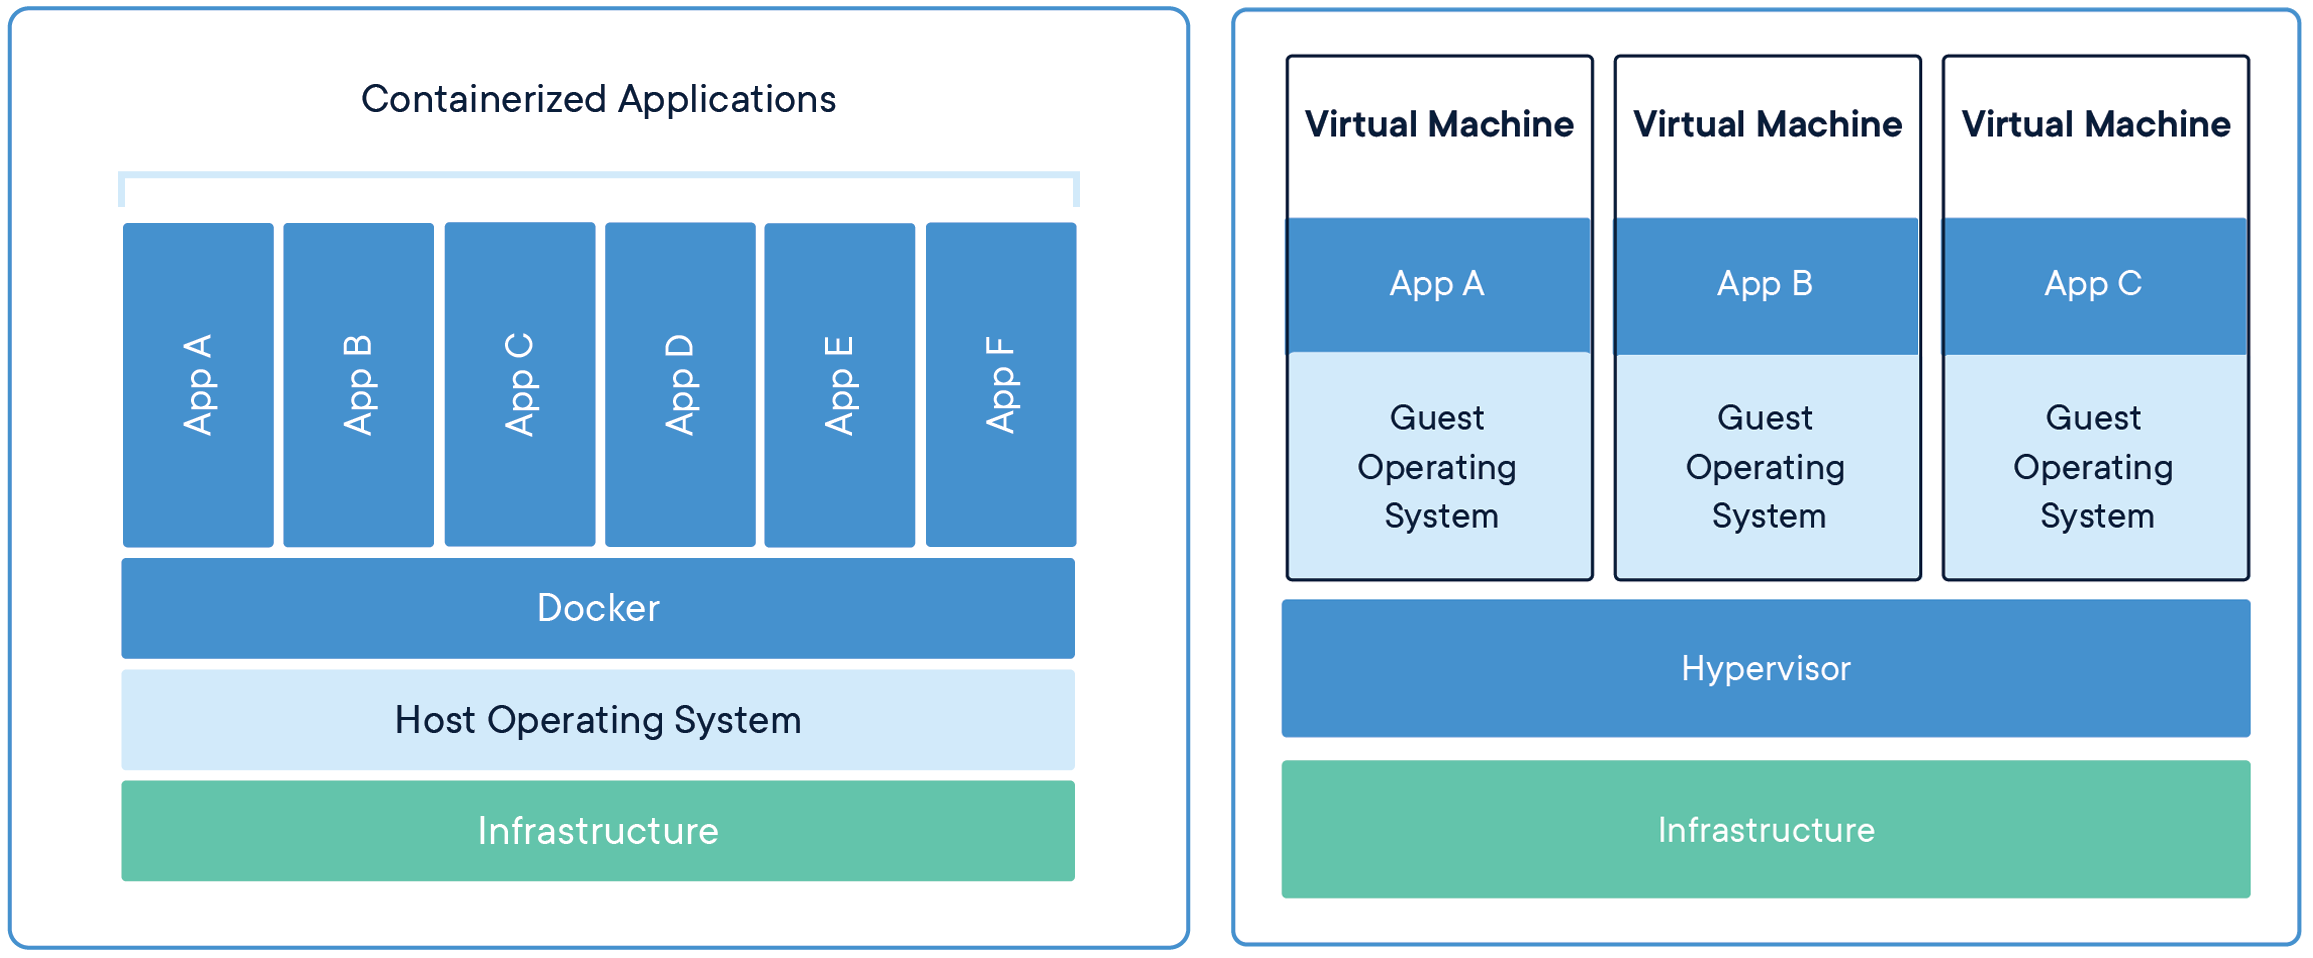
\includegraphics[width=\linewidth]{images/Virtualization-Containerization.png}
    \caption{This image comes from Docker's website\cite{docker}.}
    \label{fig:virt-vs-cont}
  \end{center}
\end{figure}

\paragraph{}Because of what they are, those two solutions usually didn't apply to the same situations.  A VM (Virtual Machine) is a much more complicated and complete structure, that takes more time to boot but provides a better isolation.  And the Container is much lighter, quicker to launch but less isolated.  Traditionally, in the Cloud Computing world, VMs rely in IaaS (Infrastructure-as-a-Service) while Containers rely in PaaS (Platform-as-a-Service).  This paper \cite{dua2014virtualization} made a detailed point about it back in 2014.

\paragraph{}But recently things started to change, some new solutions seem to have the advantage of both sides, the isolation of a VM and the portability and lightness of a Container.  This is why some VM-based solution are presented here.  Even though VMs do not come from the same domain of application as Containers, and even though in the case of INGInious, Containers were 5 years ago the obvious choice, it might now be time to reconsider it.

\section{Namespaces}
\paragraph{}Namespaces are a feature of the Linux kernel since 2002, they are a key element that made containerization possible.  A namespace can be associated to a context, which is a partition of all the resources of a system that a set of processes has access to, while other processes can't.  Those sets of resources can be of seven kinds:
\begin{itemize}
\renewcommand\labelitemi{--}
  \item \textbf{mnt} (Mount): This controls the mount points.  Processes can only have access to the mount point of their namespace.
  \item \textbf{pid} (Process ID): This allows each process in each namespace to get a process id assigned indepedently of other namespaces porcesses.
  \item \textbf{net} (Network): This provides a virtualized network stack.
  \item \textbf{ipc} (Interprocess Communication): This allows processes of a same namespace to communicate with one another, for example by sharing some memory.
  \item \textbf{uts} (Hostname): This allows to have different hostnames on a same machine, each hostname being considered as unique by the processes of its namespace.
  \item \textbf{user} (User ID): This allows to pretend to change the user in a namespace, si that it could behave like he had more privileges for example.
  \item \textbf{cgroup} (Control group): This provides a virtualization of the resources available to the processes of the namespace.
\end{itemize}

\paragraph{}When a Linux machine starts, it initiate one namespace of each type in which all the processes run.  The processes can then choose to create and switch of namespaces.

\section{Containerization solutions}

Here bellow are presented some containerization solutions.

\subsection{Docker}
\paragraph{}Docker\cite{merkel2014docker} is today probably the most known solution for containerization.  Since its apparition in 2014, its interest for the PaaS sector hasn't ceased to grow.  It is now tightly binded with Kubernetes, "an open-source system for automating deployment, scaling, and management of containerized applications" \cite{kubernetes}.  It consists in a daemon, running on the host, that allows to easily manage different containers.  It relies on Containerd, "An industry-standard container runtime with an emphasis on simplicity, robustness and portability"\cite{containerd}, which itself uses runc ("runc is a CLI tool for spawning and running containers according to the OCI specification." \cite{runc}).

The main advantages of Docker are its simplicity of use, its production-grade quality, the huge fleet of ready-to-run containers publicly available and a lot of useful tools (like \texttt{docker-compose} that come along with it).  This is the solution currently used by INGInious.

\subsection{Podman}
\paragraph{}"Podman is a daemonless container engine for developing, managing, and running OCI Containers on your Linux System."\cite{podman}  Podman present itself as a viable true alternative to Docker.  Its main difference is the fact that it runs daemonless, it runs containers as child processes, it isn't therefore based on containerd as docker is.  It can also manage pods, which are groups of containers deployed on the same machine.  Podman is an Open-Source project, and is still growing a lot, the latest version at this day (2020-02-28) is v1.8.0, released 21 days ago, and already 287 commits have been done since then!

\subsection{LXC}
\paragraph{}"LXC is a userspace interface for the Linux kernel containment features."\cite{lxc}  This solution is developed and maintained by Canonial Ltd.  Docker used to be based on LXC until it created its own execution environment.  The main difference between LXC and Docker is that LXC launches a complete Linux init for each new container, while Docker will only launch a service, the application, in the container.

\subsection{SAND} 
\paragraph{}SAND\cite{akkus2018sand} aims at improving the performance of serverless computing with two techniques: application-level sandboxing, and a hierarchical message bus.  Serverless can be seen as an improvment of Paas, with better scalability and efficiency.  It can really be associated with what INGInious does when testing a submission; it is basically, running a function, on user demand, with no direct link with the structure of the application.  The main difference between what INGInious does and what serverless offers is that usually, in serverless, you run a bunch of functions over and over again, only with different inputs.  With INGInious, the different inputs to those functions are the code of the student to execute, which makes the function execution unique for each submission.  This is still interesting to look at the improvment done in this sector though, as the underlying technology is quite similar, as it is often based on containers.  
\paragraph{} Coming back to SAND, here are the two interesting techniques they used to improve serverless computing:
\begin{itemize}
\renewcommand\labelitemi{--}
  \item \textbf{Application Sandboxing}: The key idea here is to manage differentiate multiple executions of different functions with multiple execution of a same function.  In the first case, as usual, a new container is launched on the new function demand and the function is executed inside of it.  In the second case, instead of lauching a new container with exactly the same configuration as an already running one, we only fork a process inside de running container to deal with the new demand, which is much faster than creating a new container.  The problem in our case, is that we loose the isolation between student code execution, which is not desirable.
  \item \textbf{Hierarchical Message Queuing}: The goal to this is to facilitate communication between functions that interact with one another (i.e. the output of a function is the input of another one).  To do so they use a two-level communication bus: global and local.  Global means that the communication is made between different functions on different hosts, while local means different functions on the same host.  As accessing the local bus is much faster than the global one, it can decrease latency for functions on the same host.  In our case, as INGInious is still running on a single host, this shouldn't improve our performances that much.  But in a near future where INGInious get a new horizaontally scaled architecture, it might be interesting to come back on it.
\end{itemize}

\subsection{SOCK} 
\paragraph{}Sock\cite{oakes2018sock}

\section{Virtualization solutions}

Here bellow are presented some lightweight virtualization solutions.

\subsection{Firecracker}
\subsection{Kata Containers}
\subsection{LightVM} \cite{manco2017my}

\section{Summary}
